\subsection{Les supports de communication}

\UPSTIdefinition[Support de communication]{Le support réseau désigne les éléments qui transmettent physiquement l'information (ondes électromagnétiques, fils éthernet, fibre optique, \dots)}
Pour transférer une information, il faut un support. Dans le cas d'une communication entre humain, il s'agit de l'air : les vibrations sonores se déplacent dans l'air pour parvenir jusqu'à la destination.

Dans le cas des réseaux informatiques, il existe une multitude de supports. Nous verrons ici les principaux : ceux que nous rencontrerons le plus dans ce module et ceux que l'on rencontre le plus souvent autour de nous.

\subsubsection{Les supports filaires}

\paragraph{Les câbles Ethernet}
C'est le câble le plus répandu pour relier des machines sur des réseaux de moyenne ou petites tailles.

Un câble Ethernet est un ensemble de 4 paires torsadées (Figure~\ref{fig:cableEthernet}).

Dans la configuration la plus simple, les paires oranges et vertes sont utilisées pour la tranmission des données, les deux autres paires ne sont pas utilisées.

Concrètement, lorsque deux machines sont reliées par un câble Ethernet, l'une d'elle émet sur une paire torsadée et écoute sur l'autre ; la deuxième machine fait l'inverse. Le signal Tx est utilisé pour \textbf{T}ransmettre et le signal Rx est utilisé pour \textbf{R}ecevoir. C'est pourquoi on utilise des câbles dits \textit{croisés} pour relier deux ordinateurs ensembles : Les broches Tx d'un élément sont reliées aux Rx du deuxième et inversement.

Les câbles droits sont utilisés pour relier les ordinateurs à des organes propres au réseau comme un concentrateur dont les broches Tx et Rx sont inversées.

\begin{figure}[ht]
  \centering
  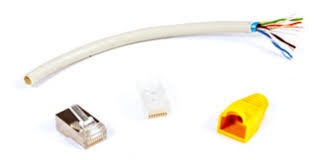
\includegraphics[width=.3\textwidth]{images/materiel/cableEthernet}
  \caption{Câble Ethernet et son interface RJ45}
  \label{fig:cableEthernet}
\end{figure}

\UPSTIremarque{On dit parfois \textit{câble RJ45}. Il s'agit d'un abus de langage car \textbf{RJ45} désigne l'interface (embout) du câble.}

\paragraph{La fibre optique}
Pour relier des réseau entre eux, on utilise de plus en plus la fibre optique. Un tel câble utilise la lumière comme moyen de propagation de l'information. Vous verrez son principe de fonctionnement plus en détail en cours de physique S3.

La fibre optique permet de bien plus forts débits qu'un cable Ethernet en cuivre (plusieurs Terabit par seconde contre plusieurs Gb/s pour un cable Ethernet). Les connexions intercontinentales sont notamment réalisé avec une fibre optique.

Comme pour un support en cuivre, la fibre optique subit une atténuation avec la distance. Afin de permettre au signal de traverser de très longues distances (l'atlantique par exemple), on pose régulièrement des répéteur qui reçoivent le signal, l'amplifient, puis le répète.

La Figure~\ref{fig:poseFibre} illustre la pose d'un câble de fibre optique sous-marin.

\begin{figure}[h]
\centering
  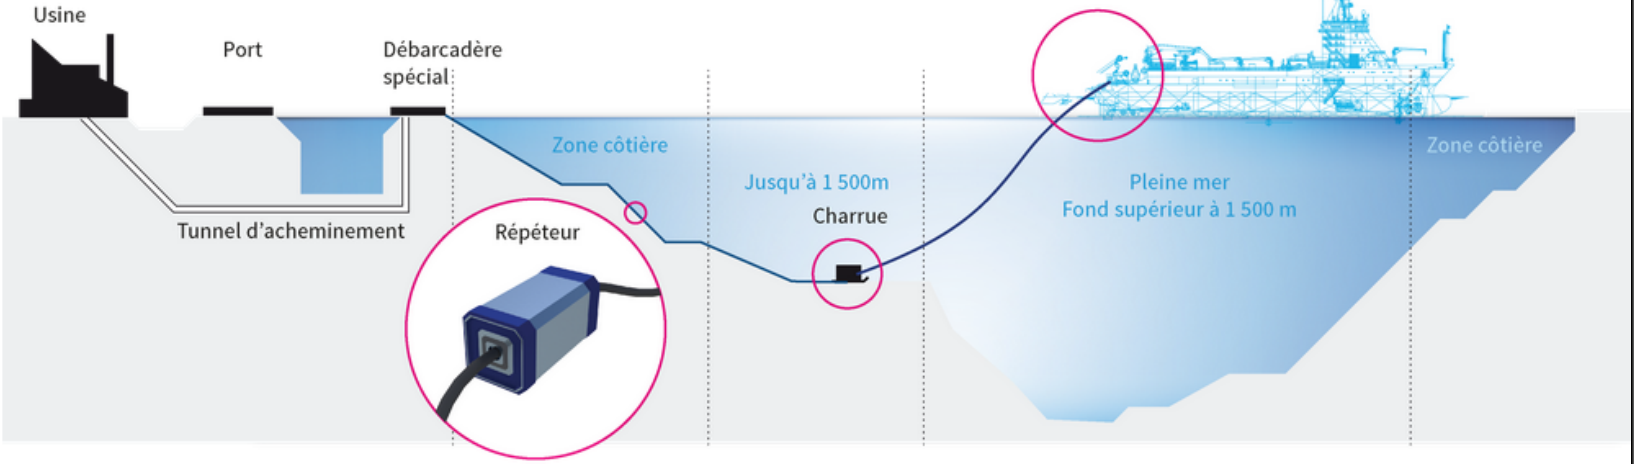
\includegraphics[width=.9\textwidth]{../../images/materiel/poseFibrecroped}
  \caption{Pose d'un câble de fibre optique sous-marin (Source : Le Monde)}
  \label{fig:poseFibre}
\end{figure}

\subsubsection{Supports sans fil}
\paragraph{Wi-Fi}
A l'échelle locale, le support sans-fil le plus utilisé est sans doute la connexion Wi-Fi. Il s'agit d'une transmission par ondes électromagnétiques à des fréquences entre \SI{2.4}{GHz} et \SI{2.4935}{GHz}.

La connexion Wi-Fi a un débit théorique inférieur à une connexion Ethernet mais permet la mobilité des organes connectés.
